%------------------------------------------------------------------------------
% No implementation, software engineering details, or project management
%------------------------------------------------------------------------------

%------------------------------------------------------------------------------

\begin{subsection}{The Elevator Pitch}
  Advances in technology have revolutionised other industries and parts of agriculture, bringing with it radically improved methods and cost efficiencies. However, the methods used to identify, catalogue, and mark cattle have remained old-fashioned and out-of-date.

  Globally, with particular focus on developing countries, cattle are revered. They often represent a high proportion of a farmer's livelihood and wealth. It is in such countries where the systems required to protect a farmer's livelihood and his cattle are at their weakest and the greatest opportunity arises for corruption and theft of cattle.

  CowHub provides access to a catalogue of cattle which can be used to for identification purposes without the need for physical deformation of the animal. In doing so, any cattle that has not been tampered with (it's muzzle) can be identified as belonging to it's owner deterministically and with near certain reliability\footnote{Whilst no statistical tests have been performed during this project, previous works have indicated that the unique identity of a cattle is tied with the biometric nature of it's muzzle}.
  % TODO: Reference to paper regarding testing of 2,500 muzzles
\end{subsection}

%------------------------------------------------------------------------------

\begin{subsection}{Project Description}
  This project will focus on providing a technology-based answer to the problem aformentioned. It will consist of the development of a user-friendly platform that uses a scalable and centralised cattle management and identification system. The three key objectives for this project are the following:

  \begin{itemize}
  	\item Offer a \textbf{harmless, physically non-destructive alternative} to current methods used to identify cattle
  	\item Provide a service that \textbf{allows the identification of cattle}
  	\item Collect data on cattle from farmers to be able to \textbf{build and use a widespread catalogue of information regarding cattle and their movements}, relating to current and future (not yet foreseen) purposes.
  \end{itemize}

\end{subsection}

%------------------------------------------------------------------------------

\begin{subsection}{What is the need for the project?}
  The process of marking cattle can be incredibly painful, regardless of the age of the cattle, and is a controversial aspect of the identification process for animal rights activists. Being subject to this pain or witnessing its offspring being subject to this the pain can be highly traumatic for a cow. Members of the public feel so strongly about the issue that protests have been made where by members of the public have branded themselves, much to the disgust of onlookers~\cite{theguardian1}.

  Whilst branding itself is no longer carried out in the United Kingdom, current methods, including piercing a cattle's ears, are still in use today and are without animal-friendly competition. Often these forms of marking or identification are aided by RFID tags on collars, and potentially chips which are ingested by the cattle allowing the cattle to be scanned.

  \begin{figure}[H]
  	\centering
    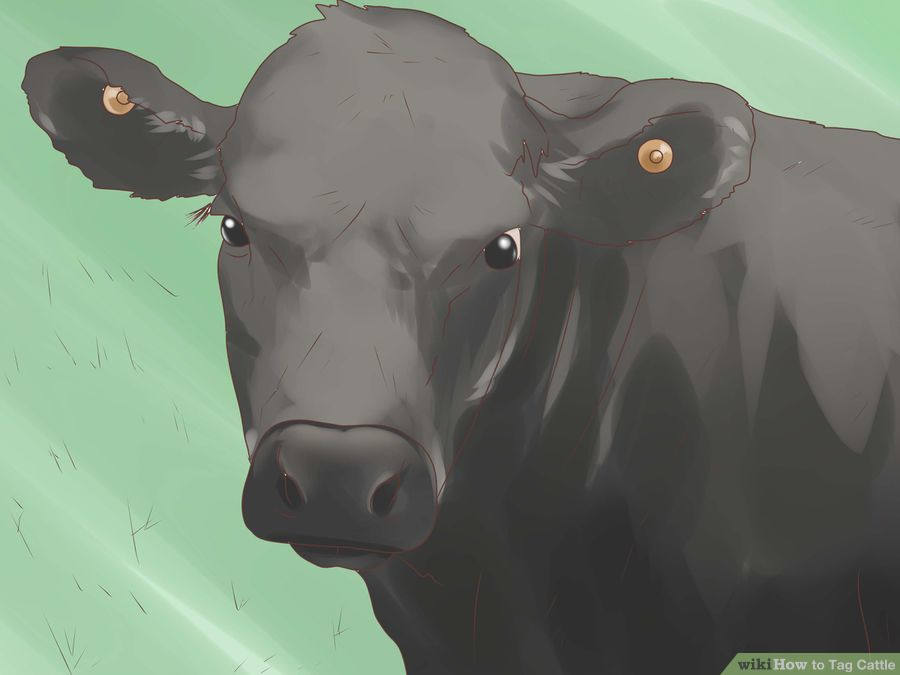
\includegraphics[width=0.5\textwidth]{images/cattle-with-ear-tag.jpg}
  	\caption[Cattle ear tagging]{
      Illustration of a cattle's head, demonstrating the position and rough size of cattle tags from the front. \cite{wikihow1}
  	}
  \end{figure}

  CowHub seeks to provide a user friendly platform to easily register and manage the information of a cattle. In addition, it also offers a non-intrusive solution for cattle recognition and by doing so alleviates all tagging-associated pain from implementing the current system.

\end{subsection}
